
%(BEGIN_QUESTION)
% Copyright 2010, Tony R. Kuphaldt, released under the Creative Commons Attribution License (v 1.0)
% This means you may do almost anything with this work of mine, so long as you give me proper credit

This Siemens S7-200 PLC controls a motor contactor and a lamp from two process switches:

$$\includegraphics[width=15.5cm]{i04539x01.eps}$$

Examine this ``live'' program display for the PLC (showing colored status highlighting), determining what process condition(s) account for the lamp being energized and the motor not running:

$$\includegraphics[width=15.5cm]{i04539x03.eps}$$

\underbar{file i04539}
%(END_QUESTION)





%(BEGIN_ANSWER)

Process level being below 11 feet and process pressure being above 45 PSI accounts for all the color status highlighting we see in the program, as well as the LED statuses on the front of the PLC.

%(END_ANSWER)





%(BEGIN_NOTES)

\vfil \eject

\noindent
{\bf Prep Quiz:}

This Siemens S7-200 PLC controls a motor contactor and a lamp from two process switches:

$$\includegraphics[width=15.5cm]{i04539x04.eps}$$

Examine this offline program for a PLC (no colored status highlighting shown), determining a particular set of level and pressure conditions that could account for the lamp being energized and the motor not running:

$$\includegraphics[width=15.5cm]{i04539x02.eps}$$


\vfil \eject

\noindent
{\bf Prep Quiz:}

This Siemens S7-200 PLC controls a motor contactor and a lamp from two process switches:

$$\includegraphics[width=15.5cm]{i04539x04.eps}$$

Examine this offline program for a PLC (no colored status highlighting shown), determining a particular set of level and pressure conditions that could account for the motor running and the lamp being un-energized:

$$\includegraphics[width=15.5cm]{i04539x02.eps}$$


%INDEX% PLC, relating I/O status to virtual elements

%(END_NOTES)


